\documentclass[twoside,10pt]{article}

\usepackage[labelsep=period,textfont=it]{caption}
\captionsetup[table]{name=TABLE}
\renewcommand{\thetable}{\Roman{table}}
\usepackage{lipsum,booktabs}
\usepackage[super]{natbib}
\usepackage{lipsum} % Package to generate dummy text throughout this template
\usepackage[sc]{mathpazo} % Use the Palatino font
\usepackage[T1]{fontenc} % Use 8-bit encoding that has 256 glyphs
\linespread{1.00} % Line spacing - Palatino needs more space between lines
\usepackage{microtype} % Slightly tweak font spacing for aesthetics
\usepackage{derivative}
\usepackage[hmarginratio=1:1,top=32mm,columnsep=20pt]{geometry} % Document margins
\usepackage{multicol} % Used for the two-column layout of the document
%\usepackage[hang, small,labelfont=bf,up,textfont=it,up]{caption} % Custom captions under/above floats in tables or figures
\usepackage{booktabs} % Horizontal rules in tables
\usepackage{float} % Required for tables and figures in the multi-column environment - they need to be placed in specific locations with the [H] (e.g. \begin{table}[H])
\usepackage{hyperref} % For hyperlinks in the PDF
\usepackage{multirow}
\usepackage{graphicx}
\usepackage{amsmath}
\usepackage{amsfonts}
\usepackage{amssymb}
\usepackage{lettrine} % The lettrine is the first enlarged letter at the beginning of the text
\usepackage{paralist} % Used for the compactitem environment which makes bullet points with less space between them
\usepackage{xcolor}
\usepackage{abstract} % Allows abstract customization
\renewcommand{\abstractnamefont}{\normalfont\bfseries} % Set the "Abstract" text to bold
\renewcommand{\abstracttextfont}{\normalfont\small\itshape} % Set the abstract itself to small italic text

\usepackage{titlesec} % Allows customization of titles
\renewcommand\thesection{\Roman{section}} % Roman numerals for the sections
\renewcommand\thesubsection{\Roman{subsection}} % Roman numerals for subsections
\titleformat{\section}[block]{\large\scshape\centering}{\thesection.}{1em}{} % Change the look of the section titles
\titleformat{\subsection}[block]{\large}{\thesubsection.}{1em}{} % Change the look of the section titles

\usepackage{fancyhdr} % Headers and footers
\pagestyle{fancy} % All pages have headers and footers
\fancyhead{} % Blank out the default header
\fancyfoot{} % Blank out the default footer
\fancyhead[C]{The Ratio of Charge to Mass of the Electron $\bullet$ November 21, 2021 } % Custom header text
\fancyfoot[RO,LE]{\thepage} % Custom footer text


%----------------------------------------------------------------------------------------
%	TITLE SECTION
%----------------------------------------------------------------------------------------

\title{\vspace{-15mm}\fontsize{15pt}{10pt}\selectfont\textbf{The Ratio of Charge to Mass of the Electron}} % Article title

\author{
	\small
	\textsc{Lauren Hernandez, Kathryn Wong}\\[1mm] % Your name
	\normalsize \textit{University of Houston}\\ % Your institution
	\normalsize \textit{Physics 3313: Advanced Laboratory I}\\ % Your Course
	%	\normalsize \href{mailto:john@smith.com}{john@smith.com} % Your email address
	\vspace{-10mm}
}
\date{}

%----------------------------------------------------------------------------------------

\begin{document}
	
	\maketitle % Insert title
	
	\thispagestyle{fancy} % All pages have headers and footers
	
	%----------------------------------------------------------------------------------------
	%	ABSTRACT
	%----------------------------------------------------------------------------------------
	
	\begin{abstract}
		
		\noindent This experiment uses the Bainbridge Tube method in order to calculate the ratio of charge to mass of the electron, e/m. The ambient magnetic field was calculated to be 4.244 x 10$^{-7}$ Tesla, and the ratio of charge to mass was calculated to be 2.1811473 x 10$^{11}$ C/kg.
		
		
	\end{abstract}
	
	%----------------------------------------------------------------------------------------
	%	INTRODUCTION
	%----------------------------------------------------------------------------------------
	
	\begin{multicols}{2} % Two-column layout throughout the main article text
		
		\section{Introduction} 
		
		\lettrine[nindent=0em,lines=2]{I}n 1897, J.J. Thompson used the electron charge to mass ratio experiment to demonstrate that atoms are not fundamental units, but rather, atoms are the housing units composed of fundamental particles$^1$. The method in which J.J. conducted the e/m ratio experiment is referred to as the Bainbridge method, which utilizes electromagnetics and mechanics, and is the same method in which we use here for this experiment. The general set-up for the e/m experiment using the Bainbridge Tube apparatus is shown below in Figure 1. 
		
		\begin{figure}[H]
			\centering
			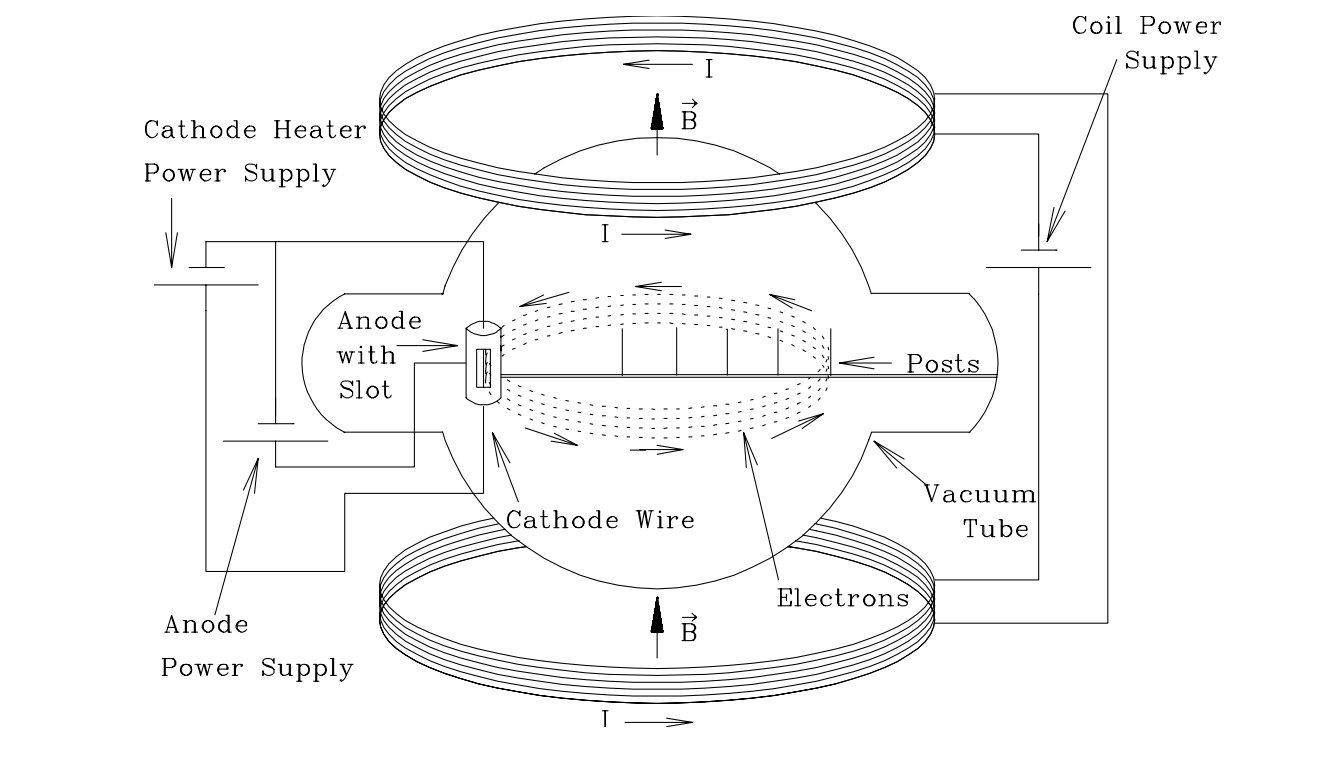
\includegraphics[width=77mm]{helmholtz coil.png}
			\caption{The Bainbridge Tube, used to accelerate an electron in a cloud of mercury vapor.}
		\end{figure}
		
		The general theory behind the experiment is that a current is passed through a tungsten filament, heating it, and causing it to emit electrons. The electrons will be accelerated by the potentential difference between the filament and the anode, which will result in a blue band, showing the path of ionization of the electrons. 
		
		In order to get an accurate calculation of e/m, the ambient magnetic field will be determined using the following equation for the magnetic field at the center of a pair of Helmholtz coils:
		\begin{equation}
			B = \frac{32 \pi \text{N} \text{I}}{5 \sqrt{5} a} \times 10^{-7},
		\end{equation}
		where B is the magnetic field, I is the current passing through the coild, N is the number of turns in the coils and a is the radius between the coils.
		
		In order to determine the ratio of charge to mass (e/m), the following relationship was made:
		
		\begin{equation*}
		 \eta = \frac{e}{m}
		\end{equation*}
	
		\begin{equation*}
		 \frac{e}{m} = \frac{v}{rB}
		\end{equation*}
		
		\begin{equation*}
		\frac{v}{rB} = \frac{ \sqrt{2 \frac{e}{m} V} }{rB}
		\end{equation*}
	
		\begin{equation*}
		 \frac{e}{m} = \frac{ \sqrt{2 \frac{e}{m} V} }{rB}
		\end{equation*}
	
		\begin{equation*}
		 \frac{e}{m} \cdot \frac{e}{m}^{-1/2} = \frac{(2V)^{1/2}}{rB} 
		\end{equation*}

		\begin{equation*}
			\sqrt{\frac{e}{m}} = \frac{(2V)^{1/2}}{rB}
		\end{equation*}

		\begin{equation}
			\frac{e}{m} = \frac{4V^2}{r^2B^2} ,
		\end{equation}

		where $eta$ represents the value of the ratio of charge, e, to mass, m. The variable $v$ represents velocity, $r$ represents the radius between the two Helmholtz coils, $B$ represents the magnetic field created by the Helmholtz coils and $V$ is the voltage passing through the coils. Equation (2) will be used to determine the ratio of e/m.
		
		%	EXPERIMENTAL PROCEDURE
		%----------------------------------------------------------------------------------------
		
		\section{Experimental Procedure}
		
		\subsection*{Equipment}
		The equipment we used for this experiment were a BK Precision Model 407F14210 multimeter, three EXTECH Instruments True RMS multimeters Model 050300047, 050500140 and EX430A, an Agilent DC Power Supply E3612A, a BK Precision DC Regulated Power Supply 1621A, an E-A Triple Power Supply EA-PS2332-025, 12 Pomona B-24 wires, a W.M Welch Scientific Co. Rheostat Resistor, a Cenco Central Scientific Co. Resistor, a Cenco 73115 meter stick, a standard dip needle,and a Cenco fine beam tube with Helmholtz coils. 

		\subsection*{Procedure}

		We set up the circuit according to Figure 2 and Figure 3 on page 2 in the lab manual$^2$. Then, we figured out the ambient magnetic field by using the dip needle, and we aligned the e/m frame to where the calculated field was axial to the coil. Then, we set the Acceleration Power Supply to 25 volts by turning the voltage knob and just barely turning the current knob to where the current was slightly greater than zero. We turned on the Filament Power Supply by turning the current all the way up and adjusting the voltage until the current was 3.8 amps. Then, we turned on the Helmholtz Power Supply by turning the voltage all the way up and turning the current to 1 amp. We turned the potentiometer on the e/m frame all the way to the right, then we let the circuit sit for approximately 10 minutes. Then, we slowly raised the Filament Power Supply current until it was just under 4.5 amps, and we adjusted the Helmholtz current by flipping the leads in the positive and negative inputs and we increades the Helmholtz current slightly in order to straighten the electron beam. Then, we adjusted the Helmholtz current to where the electron beam hit every peg on the crossbars inside the tube. We used five different voltages and all 5 pegs to determine $\eta$.
		
		%----------------------------------------------------------------------------------------
		%	RESULTS, ANALYSIS AND DISCUSSION
		%----------------------------------------------------------------------------------------
		\section{Results, Analysis, Discussion}
		
		The dip angle used to adjust the e/m frame was measured and recorded three times, resulting in an average dip angle of 66$^\circ$.
		
		\begin{table}[H]
			\centering
			\small
			\caption{Current values of the straight electron beam, and diameter recordings of the Helmholtz coils used to calculate the ambient magnetic field.}
			\begin{tabular}{l c c rrrrrrr}
			\toprule				
			 Trial &  Current (Amps) &  Diameter (cm)\\ [1ex]
			\midrule
			1	 & 0.177 $\pm$ 0.00443 & 65.2 $\pm 0.1$\\ [1.5ex]
			2	& 0.177 $\pm$ 0.00443 & 68.9 $\pm 0.1$ \\ [1.5ex]
			3	& 0.178 $\pm$ 0.00445 & 68.8 $\pm 0.1$\\ [1.5ex]
			\bottomrule
		\end{tabular}
		\end{table}

		The uncertianty in the multimeter was used for the current values, and the uncertianty in the meter stick was used for the diameter values in Table 1. The ambient magnetic field was calculated using equation 1 and was found to be 4.244 x 10$^{-7}$ Tesla. We noted that the ambient magnetic field does not oppose the applied field; the applied field aids the ambient magnetic field, which is why we had to switch the leads on the Helmholtz Power Supply in order to pivot the blue electron beam to the left (opposite the direction it was initially going in) until it was straight.  
		
		\begin{table}[H]
			\centering
			\small
			\caption{Five different current measurements taken for five different voltage readings, all data is from peg 5.}
			\begin{tabular}{l c c rrrrrrr}
				\toprule				
			Voltage &  $I_1$ (A) & $I_2$ (A) & $I_3$ (A) & $I_4$ (A) & $I_5$(A) \\ [1ex]
				\midrule
				25 V	 & 0.726 & 0.726 & 0.727 & 0.726 & 0.727 \\ [1.5ex]
				45 V	& 1.501 & 1.501 & 1.501 & 1.501 & 1.501  \\ [1.5ex]
				30 V	& 1.236 & 1.235 & 1.236 & 1.236 & 1.236  \\ [1.5ex]
				35 V	& 1.236 & 1.236 & 1.235 & 1.236 & 1.236 \\ [1.5ex]
				40 V	& 1.374 & 1.374 & 1.374 & 1.374 & 1.374 \\ [1.5ex]
				\bottomrule
			\end{tabular}
		\end{table}
		
			\begin{table}[H]
			\centering
			\small
			\caption{Five different current measurements taken for five different voltage readings, all data is from peg 4.}
			\begin{tabular}{l c c rrrrrrr}
				\toprule				
				Voltage &  $I_1$ (A) & $I_2$ (A) & $I_3$ (A) & $I_4$ (A) & $I_5$(A) \\ [1ex]
				\midrule
				25 V	 & 1.240 & 1.241 & 1.241 & 1.241 & 1.241 \\ [1.5ex]
				45 V	& 1.587 & 1.584 & 1.588 & 1.590 & 1.587  \\ [1.5ex]
				30 V	& 1.371 & 1.371 & 1.371 & 1.371 & 1.371  \\ [1.5ex]
				35 V	& 1.449 & 1.448 & 1.448 & 1.449 & 1.449 \\ [1.5ex]
				40 V	& 1.549 & 1.549 & 1.549 & 1.549 & 1.549 \\ [1.5ex]
				\bottomrule
			\end{tabular}
		\end{table}
	
		\begin{table}[H]
		\centering
		\small
		\caption{Five different current measurements taken for three different voltage readings, all data is from peg 3.}
		\begin{tabular}{l c c rrrrrrr}
			\toprule				
			Voltage &  $I_1$ (A) & $I_2$ (A) & $I_3$ (A) & $I_4$ (A) & $I_5$(A) \\ [1ex]
			\midrule
			12 V	 & 1.266 & 1.207 & 1.235 & 1.207 & 1.236 \\ [1.5ex]
			45 V	& 1.590 & 1.590 & 1.591 & 1.590 & 1.590  \\ [1.5ex]
			30 V	& 1.588 & 1.587 & 1.588 & 1.588 & 1.588  \\ [1.5ex]
		
			\bottomrule
		\end{tabular}
	\end{table}

			\begin{table}[H]
			\centering
			\small
			\caption{The radii for each peg on the nickle staff.}
			\begin{tabular}{l c c rrrrrrr}
				\toprule				
				Peg 1  &  Peg 2  & Peg 3  & Peg 4  & Peg 5 \\ [1ex]
				\midrule
				0.065 m 	 & 0.078 m & 0.090 m & 0.103 m & 0.115 m  \\ [1.5ex]
				
				\bottomrule
			\end{tabular}
		\end{table}
		
		When recording data for the value of e/m, we ran into a limitation to where we could not collect any current data that correspond to the selected voltages for pegs 1, 2 and part of peg 3. The current on the Helmholtz Power Supply had maxed out at peg 3, set to voltage 30V, and would not exceed the value of 1.588 Amps. The limitation on the current could have been due to an error in setting up the circuit; specifically, it was most likely due to the rheostat resistors. We think it was due to the resistors, because we had arbitrarily selected a specific resistance on the rheostats and we neglected to adjust them further once we started to collect data. It is possible that we set either or both rheostats to a resistance, or a cumulative resistance, that impeded our ability to exceed a fixed current on the Helmholtz Power Supply, and thus, preventing us from gathering data. Additionally, Lilly had to come help us several times, because the Acceleration Power Supply was not holding a constant voltage reading of 25 V. At various points in the experiment, the Acceleration Power Supply would deviate by up to 10 Volts at times. In these circumstances, Lilly would instruct us to check the connections between the wires and the power supplies, and we would also reset the entire circuit at times. This strange behavior in the circuit could have contributed, or could have been related to, the difficulty we had when trying to collect current readings beyond 1.588 Amps. 
		
		The ratio of charge to mass, e/m, was calculated to be 2.1811473 x 10$^{11}$ C/kg. The accepted value of charge to mass is 1.758820 x 10$^{11}$ C/kg$^3$.
		
		%----------------------------------------------------------------------------------------
		%	CONCLUSIONS
		%----------------------------------------------------------------------------------------
		\section{Conclusion}
		This experiment uses the Bainbridge Tube method in order to calculate the ratio of charge to mass of the electron, e/m. The ambient magnetic field was calculated to be 4.24 Tesla, and the ratio of charge to mass was calculated to be 2.1811473 x 10$^{11}$ C/kg. 
		
		
		
		%	REFERENCE LIST
		%----------------------------------------------------------------------------------------
		\begin{thebibliography}{99} % Bibliography - this is intentionally simple in this template
			\raggedright
			\bibliography{mybib}
			\begin{small}
				\bibitem[1]{2001}
				Electron charge-to-mass ratio - physics@brock. Electron e over m. (n.d.). Retrieved November 21, 2021, from https://www.physics.brocku.ca/Courses/1P94/lab-manual/Electroneoverm/electroneoverm.pdf. 
				

				
				\bibitem[2]{2002}
				Ulinski, A. \& Forrest, R. L., "Lab Manual for Advanced Laboratory I", Physics 3313, \textit{Determination of the Ratio of Charge to Mass for the Electron: Bainbridge Method}, pages 1 - 4, (The University of Houston, 2021).

			\bibitem[3]{2003}
				Determination of E/m for the electron. (n.d.). Retrieved November 21, 2021, from https://www.webassign.net/question\_assets
				/unccolphyseml1/lab\_4/manual.html#:~:text=In
				\%20this\%20experiment\%20you\%20will,\
				\%C3\%97\%201011\%20C\%2Fkg. 
				
			\end{small}
			
			
		\end{thebibliography}
		
		%----------------------------------------------------------------------------------------
		
	\end{multicols}
	
\end{document}